snake surrounding stuff

visual hull

salient geometric features for matching

DIVIDE TO image acquisition, reconstruction, postprocessing/rendering
ALSO FURTHER AS theory, previous work, previous usage

Close range photogrammetry, stereopsis, isolated object, camera resectioning


previous usage in:

	rockstar games / la noire; camera pairs

	polar express / sony imageworks

	ea sports / faro


surface vs motion capture

lab environment

other uses - street view, autom driving, geodetic systems

% Aikaisempi tutkimus
\section{Background}

(Should the subsections here be separated into several other sections instead of a single big ``background''?)

(corresponding problems in e.g. autonomous driving or harvester machines?)

(any point in outdoor methods?)

Pairs vs overlap? bradley: pairs

NASA cams

Perf of cloth animation capture

(Crosseyed stereoscopy, how works)

Weak perspective x=fX/Z
Ideal pinhole model projects an image upside down on its film.

\subsection{Imaging} \label{sec:imaging} % {{{
%In addition to multiple cameras at different locations and poses, an uniform lightning is also required to minimize specular difficulties in the texture.

Digital stereo vision in the end analyses digital images; this section introduces the basic image acquisition steps and concerns that affect reconstruction quality. Cameras are never ideal, and practical algorithms take lens imperfections into account (e.g. \cite{opencv}). Images are commonly taken with digital cameras that project a three-dimensional view from a single viewpoint to an image plane, and finally to a discrete grid of numerical values that describe light intensities.

Practical details, such as depth of field, sharpness, aberrations and others are not considered, as they vary greatly depending on the used hardware and are out of scope of this work.
It suffices to say that in a practical system the choice of good optics is a key to good quality reconstruction.
Accuracy and errors depend on not only decidable physical parameters of a stereo imaging rig, such as camera positioning, but also on e.g.~physical construction errors, lens imperfections, camera sensor noise, image compression and algorithmic accuracy. \cite{hollsten2013imagequality, kyto2011method,rieke2009evaluation}.

%In addition to plain photographic cameras, reconstruction can be done using e.g. laser scanners or light field cameras. Those are not covered in this work.

% }}} imaging

\subsubsection{Pinhole camera} \label{sec:pinhole} % {{{

\simplegfx{h}{0.6\textwidth}{pinhole-camera}
{Pinhole camera principle. The box represents a camera; image seen through the small hole is formed to the plane on its back, rotated upside down.}

A physical camera is in its simplest form modeled as a pinhole camera; an ideal device that projects an image upside down on its film through a small aperture.
Illustration given in image \ref{fig:pinhole-camera}.
In computer vision, this projection is given as a $3 \times 4$ matrix, when homogeneous coordinates are used.
Homogeneous coordinates add an extra dimension to the interpretation of coordinates and each point becomes a line that crosses the origin in a dimension one higher than the original.
In addition, several vector operations become more convenient to manipulate. \cite{hartley03multiview,heyden2005multiple}

The pinhole model (or, perspective projection) states that the world point $(x, y, z)$ is projected to the image plane ($f$ units away from the origin) at $(u, v)$:

\begin{equation}
\begin{pmatrix}
u \\ v
\end{pmatrix}
=
-\frac{f}{z} \begin{pmatrix}
x \\ y \\ z
\end{pmatrix}
\end{equation}

Light rays travel through the pinhole camera's aperture to the image plane that is $f$ units behind the pinhole.
The result can be derived from similar triangles with a common vertex at the aperture.
Sometimes the sign is inverted, which results in a plane between the pinhole (i.e.~camera origin) and the actual point, where the image is not rotated; this can be more convenient to analyse.
\cite{hartley03multiview}

Setting the camera to origin and using homogeneous coordinates, the mapping is given with a camera matrix as

\begin{equation}
\begin{pmatrix}
u \\ v \\ 1
\end{pmatrix}
=
\begin{pmatrix}
x \\ y \\ z/f
\end{pmatrix}
=
\begin{pmatrix} \label{eq:cmat}
	1 & 0 & 0 & 0 \\
	0 & 1 & 0 & 0 \\
	0 & 0 & 1/f & 0
\end{pmatrix}
\begin{pmatrix}
x \\ y \\ z \\ 1
\end{pmatrix}
\end{equation}

The camera position and rotation in a global coordinate frame can be encoded in a matrix so that the point $(x,y,z)$ in global coordinate frame is first transformed relative to the camera's origin; section \ref{sec:coord} discusses this in more detail.

% }}} pinhole

\subsubsection{Optics} % {{{

In practice, no actual camera works ideally; imperfections in the lenses project points to positions that differ from those predicted by straight lines in this linear case.
Lens distortions deviate the rays, and no system is in perfect focus, so that one light ray spreads out as a circle.
In reconstructing, methods that estimate the points and minimize errors are used, as no model predicts the camera perfectly.

Construction of optical systems is well studied. \cite{kingslake1989history}
Actual camera lenses consist of not only a single glass element but many, especially in the case of zoom lenses. In this work, the inner workings of these systems are ignored and equations assume a simple projective model, which is a safe assumption when the image is in focus.

The following equation applies for a thin lens while capturing sharp images:

\begin{equation}
	\frac{1}{a} + \frac{1}{b} = \frac{1}{f} \label{eq:focal}
\end{equation}

where f is the focal length of the lens, a is the distance between the lens and the film, and b is the distance between the lens and the imaged source. Figure \ref{fig:focal} example.

% TODO: fig:focal

%The focal length has a direct influence to field of view, as given in figure TODO. Longer focal length (long-focus lens, often referred to as telephoto lens) results to a more zoomed in picture, as opposed to a wide-angle lens. 

All practical optical systems (lenses) introduce some non-linear distortion that affects the performance of the ideal pinhole model.
Common distortions are the purely radial so-called barrel and pincushion distortions, where the magnification is a nonlinear function of image ray distance from the center of the lens. % XXX brown model somewhere here
Fisheye lenses are commonly known to have this kind of effect.
Tangential distortion is less common, particularly in great magnitudes, and is often ignored. Its cause is small misalignments in separate elements in a single optical system; lenses being offset from each other and not parallel to the image plane. \cite{kingslake1989history}

Wilson \cite{wilson2004anton} discusses optical systems' relation to depth of field, focus and distortions.

It should be noted that the nonlinear optical distortions are different from the inevitable perspective projection distortion that happens when projecting a 3D scene to a 2D plane, which is taken into account in the reconstruction.
Perspective distortion refers to the illusion that actual parallel lines would not be parallel in a projected image. \cite{SOMEONE}

\simplefig{h}{%
\includegraphics[width=0.2\textwidth]{gfx/barrel-distortion}
\includegraphics[width=0.2\textwidth]{gfx/pincushion-distortion}
}{fig:distortions}
{Barrel (left) and pincushion distortions that would show up in an image of a grid of straight lines. For a lens with no distortion, the lines would not be curved.}

Distortion should be corrected in software, as the following stereo algorithms assume that the images are free of nonlinear errors, i.e. straight lines in the world should remain straight in 2D images after the projective transformation.
%In particular, image rectification (discussed later in \ref{sec:rectification} won't work if this straightness does not remain; the assumption that similar features should be found on horizontal lines wouldn't hold on distorted images. \cite{hartley03multiview} 

The radial correction used by the OpenCV library to create a new image of the original pixel values at new positions \cite{opencv} is % FIXME brown model

\begin{align}
	x_{corr} &= x(1 + k_1 r^2 + k_2 r^4 + k_3 r^6)\\
	y_{corr} &= y(1 + k_1 r^2 + k_2 r^4 + k_3 r^6)
\end{align}

% (XXX some software does this in a different way (inverse of this, maybe?)

% TODO: illustrate pixel movements, such as in a vector field likein matlab toolbox

Trucco and Verri \cite{trucco1998introductory} use only the two first coefficients. For tangential distortion:

\begin{align}
x_{corr} &= x + (2 p_1 x y + p_2 (r^2 + 2 x^2))\\
y_{corr} &= y + (2 p_2 x y + p_1 (r^2 + 2 y^2))
\end{align}

$x$ and $y$ are the original coordinates in the distorted image, $x_{corr}$ and $y_{corr}$ are the corrected ones, $k_1$, $k_2$, $k_3$, $p_1$ and $p_2$ are coefficients specific to the distortion, and $r$ equals to the distance to image center located at $(x_c,~y_c)$:

\begin{equation}
r = \sqrt{(x - x_c)^2 + (y - y_c)^2}
\end{equation}

%---

Perspective distortion something something viewer location. Normal TV is usually watched at the distance of twice the screen diagonal. At this location, the scene looks normal when taken with a normal lens. A wide-angle scene then looks normal when viewed at a nearer distance. \cite{wilson2004anton}

% 14:01:55 <naavis> Kai sillä yritetään emuloida sitä, että katsojan paikalta se leffan kuvakenttä vastais sitä että valkokankaan tilalla on ikkuna.

% TODO: custom tikz for exactly specified parameters in barrel/radial

TODO: example pic of a fisheyed image and undistorted one.

% \subsubsection{Aperture}

A few words about aperture size, pixel size, diffraction limits, airy disks, circle of confusion, rayleigh limit

a real lens system with several individual elements

stabilisation lens

% }}} optics

\subsubsection{Image sensors} % {{{

compare to film

photons in, electrons out

array

Microlenses/microfacets

CCD (Charge-coupled Device)

Global shutter

CMOS (Complementary Metal-Oxide Semiconductor)

Cheaper, rolling shutter: reading the pixels out happens linearly

General image quality (noise etc.)

image stabilisation

dust reduction with vibration

%\subsubsection{Bayer filter}

\simplefig{h!}{\bayer{0.7}}{fig:bayerpattern}
{A small subsection of the repeating Bayer pattern, not drawn fully for better visualization. Each square is a single pixel; the grey area represents the image sensor. The gap between pixels is nonzero.}

Physical pixels cover less than the full area of a sensor, as there are gaps between them.

% }}} image sensors

\subsubsection{Shutter} % {{{

Mechanical vs. electrical. varying ccd charge time. mechanical moves parts and is slow, wears out. ccd shutter.

Shutter vs frame rate. More discussed in the section \ref{sec:video}. Shutter duration that exposes half of the frame time is common in professional motion pictures \cite{wilson2004anton}. While the shutter is closed, the film advances to next frame (in mechanical cameras). Blur makes the human mind think that the movement is smooth. When sampling for 3D reconstruction, the ideal shutter speed would be infinitesimally fast to reduce blur. Movement in between is then interpolated.

Flash visibility, short flash, flash shared to two frames, X-sync, ISO speed

Image upside down on the sensor, curtain goes physically from top to bottom

moving the curtain back up, springs? too much detail.

Shutter lag (auto exposure/focus even in manual mode maybe?); consistent or not? sensor sensitivity initing lag?

% }}} shutter

\subsubsection{Light sources} % {{{

Area lights, flood flashes around the target

As much light as possible but eyes gonna hurt

dark contact lenses if available (remedy)

bodies' own flashes maybe not uniform enough; too many flashes i guess

softbox or umbrella

light power vs. area, specular lobe and surface properties

%\subsubsection{Specular highlights}

Polarization filter

% }}} light sources

\subsubsection{Image download} % {{{

USB hub(s) because N cameras, single laptop

speed calculations, 20+ MB RAW vs fps vs camera buffers vs usb bandwidth vs separate hubs

usb bulk transfer protocol overhead! how many percents?

% }}} image download

\subsection{Video} % {{{

Video is consecutive, ordered pictures displayed one after another.

Hox ALL-I (intra) vs. IPB (intra-predict-bidirpredict)

Humans perceive motion when a previously seen object is seen again in a nearby location or similar position.
Current digital video technology encodes motion in a sequence of still images, usually displayed in constant rate.
Three dimensional motion is usually no different: it is encoded as discrete poses in sequence.
In order to do object capture in stereo, video material from two or more of cameras is used to initially capture a sequence of still photos.

When scanning a scene continuously, a camera grabs frames using the same principles as in photos, but does it in sequence, at a speed that is called frame rate.
Another notable point from the capture viewpoint is the shutter speed; in movies, the shutter is often open deliberately so long that fast motion is blurred, because it is considered aesthetically pleasing to human eye; even though the motion is blurred, more information about the scene movement is encoded per frame than when grabbing infinitesimally short times.
\cite{wilson2004anton}
For sharp images that are preferred in reconstruction, this is to be avoided.

\subsubsection{Frame rate effects}

More fps = better movement stopping (less motion blur), need also more light or more sensitive sensors. More sensitivity often means also more noise. Noise vs. motion blur trade-off.

Interlaced video = twice the amount of *pictures*, two pictures per frame

Film: 24 FPS traditionally

PAL. 25 FPS (50 Hz line current frequency in Europe)

NTSC. 30 FPS (60 Hz line current frequency in the US)

Actual FPS in camcorders is slowed down by a factor of 1.001 because of historical reasons relating to black and white / color TV backwards compabilities [REF].
30 and 24 FPS refer often actually to approximately 29.970 and 23.976 FPS, respectively.

24 frames per second is often transformed to 30 by carefully repeating some frames [REF].

Externally triggered cameras can be configured to record at any arbitrary speed, as long as it's in the limits of the camera speed capabilities.

\subsubsection{Frame rate vs. shutter speed}

Picture:

\begin{verbatim}

   those bars are actually just 1 pixel markers when shutter opens
   v   v   v ...

shutter
speed
1/30   |---|---|---|---|---|---|---|---|---|--- full block
1/60   |-- |-- |-- |-- |-- |-- |-- |-- |-- |--
1/90   |-  |-  |-  |-  |-  |-  |-  |-  |-  |-

   0   1   2   3   4   5   6   7   8   9

30 FPS, 10 frames = 1/3 s
\end{verbatim}

Nyquist-Shannon sampling theorem, what happens when shutter is closed, motion stopping, how eyes like blurred fast motion (more information about movement, less precise by time) [CITE slowmovideo]

\subsubsection{Multi-camera synchronization}

Multi view imaging poses lots of challenges, sync is an important one

Time offset / drift / jitter / lockstep

Offset: Different cameras do not start recording immediately at the same time, which results in one or more cameras being a little late at every frame.

Drift: A camera does not record at exactly the advertised speed, e.g. one camera's internal clock is sligtly faster than that of another.

Jitter: the difference between frames for a same camera might not be exactly the same during recording, but a more or less random delta time is added to each delay.

Le pic:

\begin{verbatim}
Offset

cam A  |   |   |   |   |
cam B   |   |   |   |   |
   0t  1t  2t  3t  4t time -->


Drift

normal   |   |   |   |   |   |   |
drifting |    |    |    |    |    |
	 0t  1t  2t  3t  4t  5t  6t time -->


Jitter

normal   |   |   |   |   |   |   |
jitterin |    |  |   | |      |    |
	 0t  1t  2t  3t  4t  5t  6t time -->
\end{verbatim}

In the scope of this paper, we consider drift and jitter negligible.
Offset may be recovered by several means.
Often used techniques are starting flash (does not need an audio track) [REF], clapperboard [REF], strobe sync'd to fps, genlock.

TODO: investigate if the errors have been researched or if they are meaningful at all.

Synchronizing all the cameras that shoot the same scene might not a trivial issue in practice, depending on the gear used.
Professional grade cameras can be synced to a single clock generator, so that they all operate on the same frequency and phase.
The same method is used when shooting with machine vision cameras that have external trigger input.
This still leaves a small phase difference caused by unequal transmission paths from the clock generator.
Synchronizable camcorders are very expensive, though, and consumer-grade hardware usually lacks all possibilities to properly sync frequency or phase, not to mention frequency drift or frame jitter.
Clapperboard is a ubiquitous and simple way to sync video and audio, but it still leaves a maximum of half a frame lag between the camera sequences; this is illustrated in figure \ref{fig:syncproblems}.
When cameras open their shutter in a different time, they effectively shoot a different scene, breaking one of the most fundamental assumptions of stereo vision: that the images encode geometrically same objects.
This can be compensated to some degree with optical flow \cite{bradley2009synchronization}.

\simplefig{h!}{
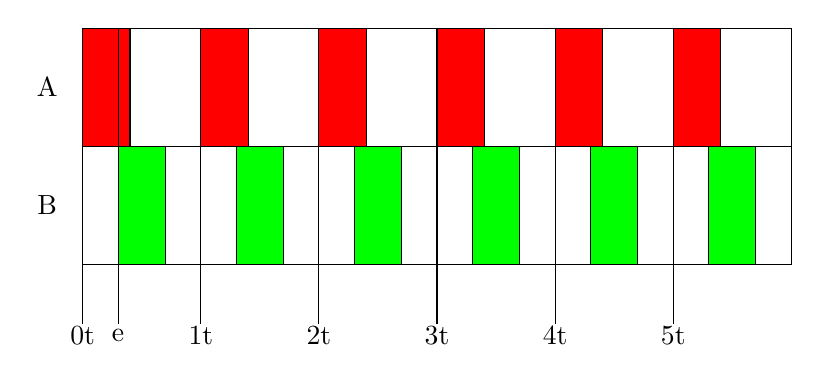
\begin{tikzpicture}[scale=1.5]
	\draw (0,0) rectangle (6,-1);
	\draw (0,-1) rectangle (6,-2);
	\foreach \x in {0,...,5} {
		\draw (\x*1, 0) -- (\x*1, -2.5);
		\node at (\x*1, -2.6) {{\x}t};

		\draw [fill=red] (\x*1, 0) rectangle (\x*1+0.4, -1);
		\draw [fill=green] (\x*1+0.3, -1) rectangle (\x*1+0.3+0.4, -2);
	}
	\draw (0.3, 0) -- (0.3, -2.5);
	\node at (0.3, -2.6) {e};
	\node at (-0.3, -0.5) {A};
	\node at (-0.3, -1.5) {B};
	% P, Z
\end{tikzpicture}
}{fig:syncproblems}
{Video phase difference.
Red rectangles illustrate exposure times of camera A, green rectangles the same for camera B.
Frame period is t, and the cameras have a constant exposure time offset of an arbitrary e.}

Faster frame rate encodes information more often, which is preferable as longer distances of pixels of same objects are more difficult to match when tracking objects; faster shutter speeds help to reduce motion blur.
Fast shutter (i.e.~short exposure) obviously needs to be compensated by using more sensitive sensors or more light to get equivalently bright images.
Noise vs. motion blur is a common tradeoff that has to be made when building a stereo vision system.

Video recording and motion tracking are best considered orthogonal issues; while a single static case can be scanned in three dimensions, so can be also each frame of a sequence, separately.
While this sounds tempting, it might not be computationally feasible, though, because the reconstruction must be started all over again for each frame and the topology is uncorrelated between the frames.
% Assumptions that the scene is locally almost the same can help and speed up computations. [?]

%Section \ref{sec:tracking} will 

\subsubsection{Video encoding}

raw video = such size wow very bloat

compression artifacts

% }}} video

\subsection{Camera selection} % {{{

general HW availability and ease of use and customizability and price

Good: Smaller sensor; smaller focal length; closer to target; less camera position disparity; smaller rig

Image quality: lens quality, sensor size, pixel count, lighting

Common sensor sizes in dslr cameras

Common sensor sizes in pocket cameras

Canon / Nikon dslr

% http://www.agisoft.ru/forum/index.php?topic=1411.60

lens sharpness, contrast, freq; MTF modulation transfer function for the lens sharpness / perceptual mpix

fixed lens (prime) instead of zoom: more or less lab controlled environment -> target position can be adjusted, zoom would be just more parameters to optimize. focal length is important to know; also, mirror vibration might move the zoom over time.

no anti-shake/image stabilizer  (photogrammetry.doc) in sensor or lens

Rieke-Zapp et al \cite{rieke2009evaluation} address several problems in camera calibration and imaging quality, e.g. mechanical problems blah blah

sensor vibration to remove dust -> sensor position not very fixed (rieke2009) % TODO MEASURE!

ring flash bending the lens assembly if attached to it (rieke2009)

\subsubsection{DSLRs}

Intended for single pictures

Mechanical shutter

Big sensor

Shallower DOF

Focal length configurable

Lots of resolution

Memory card speed

gphoto2

No autofocus in general

Easy sync for single image

\subsubsection{Pocket cameras}

Affordable

Small sensor

Decent resolution

Configurability unknown

Manual mode required

Always a zoom lens, bad for calibration

\subsubsection{Camcorders}

Electrical shutter

Ok fps

More features for video

Autofocus (not needed here)

Better (deeper) DOF for video

Usually zoom lens

Consumer devices: affordable

Pro devices: bukkits of money (features; external sync)

Internal hard disk

Interlace vs. progressive recording

\subsubsection{Webcams}

Like camcorders but shit, only good feature is their price

closed design, poor manual settings

\subsubsection{Machine vision cameras}

Well controllable, flexible (in SW terms), still vendor-specific APIs for tuning the settings (as is with any other vendors too, but no good general-purpose libs for these as opposed to gphoto2 due to high price = bad availability for consumers; should afford extra time for coding too)

External sync

Raw data

Data bandwidth, auxiliary hardware

Expensive

- vendor-specific apis
- probably easier to control
- expensive
- raw images (high bandwidth)
- usually fixed lens
\subsubsection{Depth cameras}

In addition to stereo depth...

Active measurement (difficult to use several)

Laser rangers

IR patterns and an IR camera (Kinect)

\subsubsection{(Light field cameras)}

Lytro (NOPE)

\subsubsection{Hybrid systems}

Use several camera types at the same time? depth camera for more reliable and fast measurements? not really done, should we try it?

% }}} camera selection

\subsection{Hardware} % {{{

do i need this section?

\subsubsection{Image storage}

memory cards and all that (lots of this is discussed above, though)

Integral memory cards / disks, offline usage

memory cards cannot be swapped out because of simply too much manual work

\subsubsection{Transport buses and cabling}

USB2

USB3

Firewire

GigE

Camera Link

libgphoto2; googl others for machine vision

\subsubsection{(Mechanical something)}

support structures out of bounds; just assume that the construction is rigid enough?

% }}} hardware

\subsection{Static 3D reconstruction}

% TODO: combine and structure better the following flattened section list
% TODO: intro paragraph(s)

\subsubsection{Imaging methods} % {{{

% separate part or part of 3d reconst intro? or combine to intro?

some basic stuff about how 3d structure can be recovered with many different means (i.e. different camera types): light field, structured light, laser scanner, multiview stereo

- every Nth frame free of patterns for texture extraction (zhang snavely curless 2004)
- maybe not fast enough with common cameras

% }}} imaging methods

\subsubsection{Coordinate systems and transforms} % {{{

% (XXX rename?)

%Homogenous point description here, [dubrofsky] homography estimation is nice, also refer hartley/zisserman

%Homography definition (mapping of points and lines in $P^2$) / panorama homography

The previous imaging section described how to record a view of a scene with a camera. From now on, the term camera refers to a particular camera configuration, which can be a single physical camera moved to different locations.
No optical system is assumed; at this point, the camera is reduced to the pinhole model \ref{sec:pinhole}.

% FIXME: describe more of these in pinhole and less here, just recap here what pinhole describes?
% intrinsics into camera workings, join them here to extrinsics
% TODO pics, coordinate system at place,pose X vs origin (from paper notebook)

The camera is a projective object located somewhere in the imaged scene.
Its \textit{intrinsic parameters} model the properties of projection, but do not take into account the camera location in any global coordinate system.
The \textit{extrinsic parameters} contain the camera location and rotation in another global coordinate system, structured as a matrix.
This is especially advantageous when there are more than one cameras and their coordinates must be related.
\cite{hartley03multiview,heyden2005multiple}
This part quickly reviews basic transforms whose results are needed in the later reconstruction steps.

%Calibration is often specified with a camera projection matrix, or several separate matrices.
%It may be convenient to store intrinsics and extrinsics separately if the intrinsic matrix is constant for several pictures, for example.

% FIXME especially this should be elsewhere
\simplefig{h}{%
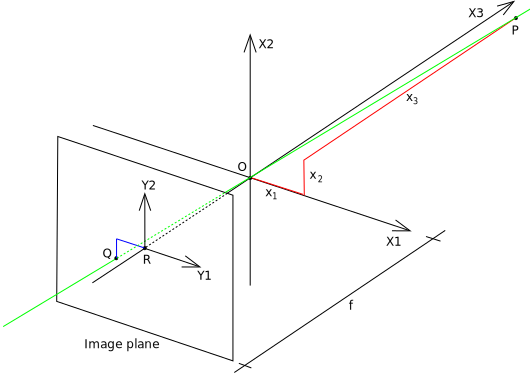
\includegraphics[width=0.7\textwidth]{gfx/pinhole3d}
}{fig:pinhole3d}
{Pinhole camera geometry. Camera coordinate system origin at O, axis X3 points towards the optical axis, Y1 and Y2 point to image plane axes and R is the principal point, at the image center. The point P projects to Q, as well as everything else on the line joining them. The image plane is f units away from camera origin; f is called the focal length.}

In computer graphics and vision, points and directions are usually described in homogeneous coordinates.
Translation, perspective projection, rotation, and other operations are conveniently described as matrices by using an additional dimension for points, of which usually the last element is 1: $(x, y, z, 1)$.
All points $(xw, yw, zw, w)$ map to the same point $(x, y, z)$.
\cite{dubrofsky2009homography,hartley03multiview}

%Homography definition (mapping of points and lines in $P^2$)

The imaging process essentially captures a projection to a flat two-dimensional plane of the camera's view, as described in section \ref{sec:imaging}.
When relating points between different cameras that view the same scene, the cameras' relational positions and rotations must be known.
One of the cameras is often conveniently chosen as the origin of a global coordinate frame, so that its extrinsic parameters become unity transforms (programming libraries often assume this, see e.g. \cite{opencv}).
Each three-dimensional point in the world is transformed to the small sensor or film inside the camera, which is then digitized to a discrete two-dimensional grid of pixels. The size of this pixel array (i.e. image) is referred to as the camera's resolution.

%Figure \ref{fig:TODO} illustrates this transformation chain, which is encoded as the following equations, given a homogeneous point (4-dimensional vector) $X$ representing a 3D location described in physical (e.g. metric) coordinates:

The transformation chain is encoded as follows, given a homogeneous point (4-dimensional vector) $X$ representing a 3D location described in physical (e.g. metric) coordinates:

\begin{align}
	x &= P X\\
	  &= M_i X_s\\ % X_s on the sensor
	  &= M T R X\\
	  &= M_i M_p T R X\\ % R, T camera pose, M_4 to camera sensor, M_3 to pixel coords
\end{align}

$x$ is a 2d pixel in a discrete image, $X_s$ exists on the sensor. $R$, $T$ encode the camera rotation and translation (extrinsics); $M_p$ projects the world coordinates to the camera sensor (film) - still in world coordinates (intrinsics!), and finally the affine $M_i$ transforms the points from the sensor to pixel coordinates on the digital discretized image.

The whole projection $P = M_i M_p T R$ can be used as-is without decomposing it to separate matrices, unless the individual parameters are needed. As the chain consists of several matrices, some of them are defined only up to scale; the coordinate systems' units can be chosen freely. Software packages usually do not decompose the chain, because it is not needed and unique parameters cannot be found because of scaling.

%The external camera parameters are called the extrinsics: camera coordinate system position and rotation (heading) in the global space.
%Camera position sits at the projection center blah.

The internal parameters, intrinsics, encode how the image is formed on the sensor: they consist of focal length, sensor size and principal point: (last column left out, as it's full of zeroes in 3x4)

\begin{equation}
	M =
	\begin{pmatrix}
		m_x & \gamma & u_0\\
		0   &    m_y & v_0\\
		0   &        0 & 1
	\end{pmatrix}
\cdot
	\begin{pmatrix}
		f & 0 & 0\\
		0 & f & 0\\
		0 & 0 & 1
	\end{pmatrix}
	=
	\begin{pmatrix}
		\alpha_x & \gamma   & u_0\\
		0        & \alpha_y & v_0\\
		0        & 0        & 1
	\end{pmatrix}
\end{equation}

For simplicity, it is often denoted $\alpha_x = m_x f$, $\alpha_y = m_y f$. $R = (u_0, v_0)$ is the image center (or principal point). For square pixels, $m_x = m_y$, and for a non-skewed sensor, $\gamma = 0$, which is often the case. \cite{hartley03multiview,szeliski10vision,heyden2005multiple}

%Le image. Horizontal planar triangle, lines between camera origins etc. lecture11.pdf.

% }}} coord systems and transforms

\subsubsection{Camera calibration} % {{{

Calibration is often specified with a camera projection matrix, or several separate matrices.
It may be convenient to store intrinsics and extrinsics separately if the intrinsic matrix is constant for several pictures, for example (?).

calibration can be automatically determined, given by X corresponding points that can be distinguished in each image and matched [?]. Commonly the points are particular \emph{features}, commonly very noticiable edges or corners, found with an algorithm such as SIFT [?], SURF [?] or Harris corner detector [?].

TODO Figure: show extrinsic in matlab cam calibs, nice pics (both cam and world centered)


%In order to accurately measure a scene with a camera, the camera's properties must be known.
Reconstruction algorithms need to relate points between images; the camera properties are needed.
Calibrating a camera means to measure its intrinsics and extrinsics in order to map its data to a known coordinate frame.
Calibration has always to be done, but it does not necessary need to be a manual step before scanning; self-calibration attempts to target this convenience problem. \cite{pollefeys1999hand,hartley03multiview}

%Projective calibration only is too general, as it leaves out some assumptions that can be done about a physical world, such as relative angles and sizes; metric calibration something something. \cite{zisserman1995metric}.

Automatic calibration tools rely on an amount of feature pairs of which the best matches are found, or a known pattern, such as a planar checkerboard pattern \cite{chuang2002performance,zhang2000flexible} whose features are also distinguished with a similar algorithm but a priori knowledge of the object structure is used for precise calibration.
These usually need several pictures taken with the same camera from different poses.

The checkerboard calibration step can also measure optical distortion at the same time. \cite{opencv,camcalmatlab}

%TODO Figure: show extrinsic in matlab cam calibs, nice pics (both cam and world centered)

%Single three-dimensional calibration object is also sufficient blbl

One possible way is direct linear transform (DLT)
\cite{hartley03multiview}: the whole matrix $P$ is solved from $x_i = PX_i$ by constructing a system of equations from the projections of some known points $i$, and minimizing an error metric, as the case is usually overconditioned.

%Methods that dig the matrix out of a single image have certain restrictions, and won't work if e.g. seven points lie on the same plane [longuet-higgins etc.]

%XXX see below. Intrinsic, extrinsic. Distortions. Projection matrices. Camera resectioning.

%many single planar chessboard pics vs. a single image of an accurate 3d model.
%Single three-dimensional calibration object is also sufficient blbl


%The scale of values in the equations above affects the precision [hartley, in defense of .., h,ziss]. A similarity transform can be used to modify the values to a more consistent range; this is called normalization of the data.

%XXX see below. Intrinsic, extrinsic. Distortions. Projection matrices. Camera resectioning.


% }}} camera calibration

\subsubsection{Normalization} % {{{

The scale of values in the equations above affects the precision \cite{hartley1997defense,hartley03multiview}.
A similarity transform can be used to modify the values to a more consistent range.

Translate centroid to the origin, scale so that average becomes sqrt 2.

maybe move this to a paragraph as part of another section.

% }}} normalization

\subsubsection{Binocular disparity} % {{{

%Essential, fundamental matrices. Correspondence problem. Rectification, undistortion. Epipolar geometry.

\simplefig{h!}{
\begin{tikzpicture}[scale=0.3]
	% P, Z
	\draw[fill] (0, 20) circle [radius=0.3];
	\node at (0, 21) {$P$};

	\draw [<->] (0, 0.5) -- (0, 19.5);
	\node at (0.5, 10) {$Z$};

	% origins, T
	% TODO: circles, node ends not exactly at those points
	\draw [<->] (-9.5,0) -- (9.5, 0);
	\draw[fill] (-10, 0) circle [radius=0.3];
	\draw[fill] ( 10, 0) circle [radius=0.3];
	\node at (-10, -1) {$O_l$};
	\node at (10, -1) {$O_r$};
	\node at (0, -1) {$T$};

	% headings
	\draw [->] (-10, 0) -- (-10, 10);
	\draw [->] (10, 0) -- (10, 10);

	% image planes, at y=4
	\draw[thick] (-13, 4) -- (-7, 4);
	\draw[thick] (13, 4) -- (7, 4);

	\draw [<->] (-6, 0.5) -- (-6, 3.5);
	\node at (-5.5, 2) {$f$};


	% intersection points at principals and xs
	\draw[fill] (-10, 4) circle [radius=0.3];
	\draw[fill] (10, 4) circle [radius=0.3];

	\node at (-10.5, 3) {$c_l$};
	\node at (10.5, 3) {$c_r$};

	\node at (-9, 5) {$x_l$};
	\node at (9, 5) {$x_r$};


	% O-to-P
	\draw (-10, 0) -- (0, 20);
	\draw (10, 0) -- (0, 20);


	% p
	\draw[fill] (8, 4) circle [radius=0.3];
	\node at (8, 3) {$p_r$};
	\draw[fill] (-8, 4) circle [radius=0.3];
	\node at (-8, 3) {$p_l$};
\end{tikzpicture}
}{fig:simplestereo}
{A very simple stereo setup, picture from above. The image planes (thick lines) are actually imaginary, as a real film in a camera would exist behind the principal point and project the image upside down, as described earlier in \ref{sec:imaging}. The coordinates exist in the world coordinate units. The symbols $O$ are the camera origins ($T$ units between each other); $c$ the principal points; $x$ the image plane coordinates of $p$ w.r.t. the principal points; and $f$ is the focal length. The unknown is $Z$, depth of point $P$.}
% this figure would need to be bigger and have also the back side planes (sensors) as opposed to the (normalized?) image planes (at f=1?)

%Next, the setup of binocular stereo vision is described. Common stereo vision rigs use the simplest possible case: two identical cameras with a fixed distance, both oriented to the same direction, parallel to the line connecting them, as in figure \ref{fig:simplestereo}.

Assuming known calibration with identical cameras (same focal length and sensor) in a setup described above, visualized in figure \ref{fig:simplestereo}, points can be triangulated as follows:

From similar triangles with a common vertex at $P$, we get (note that $x_r < 0$ as it's to the left, towards to the negative axis, from the corresponding plane's origin)

\begin{align}
	\frac{Z}{T} &= \frac{Z-f}{T - x_l + x_r} \\
	&= \frac{Z-f}{T - d}\\
	ZT - Zd &= ZT - fT\\
	Z &= \frac{fT}{d} \label{eq:z}
\end{align}

The disparity $d$ is the difference of the points in their image planes, $d = x_r - x_l$.
If the image planes would be fixed as being physically correct, in the back side of the camera origins, the focal length should be negated to keep the correct interpretation and sign because the projected physical image is mirrored in both axes. Image processing between the sensor and a picture file usually inverts this.

As the equation \ref{eq:z} shows, depth is directly inversely proportional to disparity in this simple case.
To map the depth to correct units, only focal length $f$ and the baseline $T$ are needed additionally; when using pixel coordinates instead of physical in $d$, also the pixel size should be taken into account.
All of these are encoded in the camera parameters.
Algorithms such as those in OpenCV \cite{opencv} can compute point clouds from disparity images.

% }}} binocular disparity

\subsubsection{Epipolar geometry} % {{{

\simplefig{h!}{
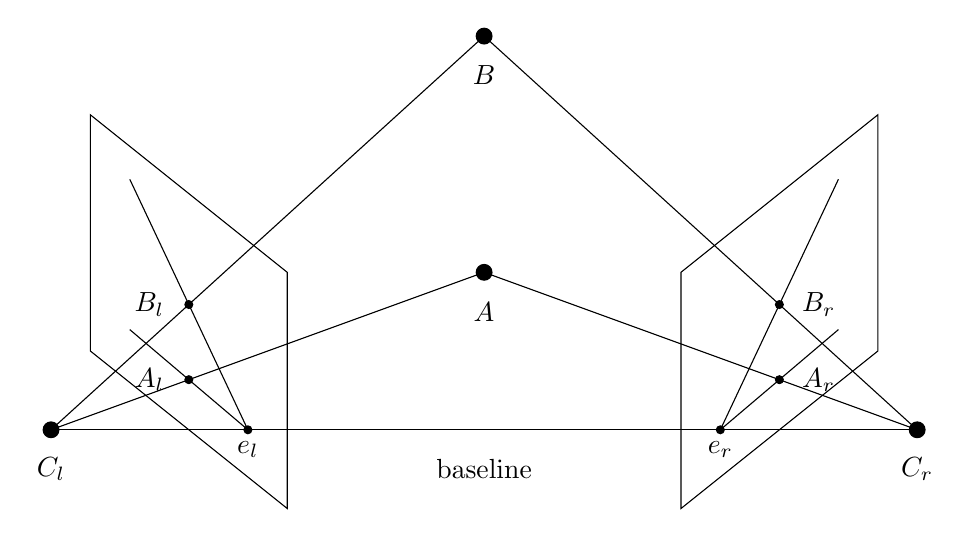
\begin{tikzpicture}[scale=0.5]
	% cameras
	\draw[fill] (-11,-1) circle [radius=0.2];
	\draw[fill] ( 11,-1) circle [radius=0.2];
	\draw (-11,-1) -- (11, -1);
	\node at (0, -2) { baseline };

	\node at (-11,-2) {$C_l$};
	\node at ( 11,-2) {$C_r$};

	% planes
	\draw (-10,1) -- (-10,7) -- (-5,3) -- (-5,-3) -- cycle;
	\draw ( 10,1) -- ( 10,7) -- ( 5,3) -- ( 5,-3) -- cycle;

	% 3d pts
	\draw[fill] ( 0,3) circle [radius=0.2];
	\draw[fill] ( 0,9) circle [radius=0.2];
	\node at (0,2) {$A$};
	\node at (0,8) {$B$};

	% origins via pts
	\draw (-11,-1) -- (0,3) -- (11,-1);
	\draw (-11,-1) -- (0,9) -- (11,-1);

	% epis
	\draw[fill] (-6,-1) circle [radius=0.1];
	\draw[fill] (6,-1) circle [radius=0.1];
	\node at (-6,-1.5) { $e_l$ };
	\node at (6,-1.5) { $e_r$ };

	% projections
	\draw[fill] (-7.5,0.2727) circle [radius=0.1];
	\draw[fill] (-7.5,2.1818) circle [radius=0.1];
	\node at (-8.5, 0.2727) {$A_l$};
	\node at (-8.5, 2.1818) {$B_l$};
	% lines from epis
	\draw (-6,-1) -- +(-2*1.5,2*1.2727);%(-7.5,0.2727);
	\draw (-6,-1) -- +(-2*1.5,2*3.1818);%(-7.5,2.1818);

	\draw[fill] (7.5,0.2727) circle [radius=0.1];
	\draw[fill] (7.5,2.1818) circle [radius=0.1];
	\node at (8.5, 0.2727) {$A_r$};
	\node at (8.5, 2.1818) {$B_r$};
	\draw (6,-1) -- +(2*1.5,2*1.2727);%(7.5,0.2727);
	\draw (6,-1) -- +(2*1.5,2*3.1818);%(7.5,2.1818);
\end{tikzpicture}
}{fig:epigeom}
{Two camera views on same scene.
World points $A$, $B$ project to planes of different views imaged from $C_l$ and $C_r$ on the left ($A_l$ and $B_l$), and to the right ($A_r$, $B_r$).
The actual images cover some area of the total projection plane, and the epipolar point may or may not lie visible in the image.
When $A_l$ is known, its corresponding point $A_r$ (not initially known in practice) is found on the epipolar line joining $e_r$ and $A_r$ in the right image.
All epipolar lines in a view join in the same point ($e_l$ and $e_r$).}
% XXX do i want the planes in physical positions too or another pic to visualize it?

% TODO: small algorithm for pairwise windowed point matching on the line (hox! and link to point matching section maybe)

% what?
Triangulation or reconstruction of the scene structure given by image pair(s) is usually done on the base of a known relationship between the cameras.
Such relationship, known as calibrating the cameras, can be automatically determined, given by corresponding points that can be distinguished in each image and matched.
\cite{trucco1998introductory,hartley03multiview}

In stereo vision, the same scene of interest is seen by two or more cameras at the same time.
The cameras are rarely aligned perfectly such as in the disparity setup described above, however.
Epipolar geometry encodes the relations between arbitrarily positioned cameras in a standard way so that coordinates of a 3D point seen in several images can be calculated with the same triangulation.

A point seen by camera $C_l$ at 3D point A could be anywhere on the line between $C_l$'s origin and P, because a certain line passing through the principal point always projects to a point.
This line is seen as a single point $A_l$.
From another viewpoint in camera $C_r$, this line equals to some line on B's image plane.
The real point must be on that line.
The inverse applies for any point on $C_r$ and a line on $C_l$.
The lines on the image planes are called epipolar lines.

% FIXME:
Essential matrix defines how the camera poses differ by the something something points seen by both.
When $A_l$, $A_r$ encode the points in figure \ref{fig:epigeom} by the corresponding camera coordinates, and the baseline difference (vector from $C_l$ to $C_r$) is marked as $t$, it holds that $(A_l-C_l) \cdot t \times (A_r-C_r) = 0$, as all the vectors are coplanar; the cross product yields a normal to the plane, which is perpendicular to all the vectors, thus the dot product equals 0.
\cite{hartley03multiview}

Essential matrix is a matrix form of this relation; it includes the relative rotation and translation of the two cameras.

%\begin{align*} \label{eq:essential}
%	%A_r &= R (A_l - t) \\
%	%A_r^T R T A_l &= 0 \\
%	%A_r^T E A_l &= 0
%	A_l \cdot t \times A_r = 0\\
%	A_l \cdot t \times R A_r = 0\\
%	A_l^T T
%\end{align*}

%where $T$ is the cross-product form of $t$ encoded in a matrix form as below. The essential matrix is obtained as $E = R T$.
%
%Le image. lecture11.pdf. O->p dot (O->O' cross O'->p') = 0
%
%Cross product expressed in a skew-symmetric matrix form is
%\begin{equation}
%\vec a \times \vec b =
%\begin{pmatrix}
%	 0   & -a_z &  a_y\\
%	 a_z &  0   & -a_x\\
%	-a_y &  a_x & 0
%\end{pmatrix}
%\begin{pmatrix}
%	b_x\\b_y\\b_z
%\end{pmatrix}
%= \vec c
%\end{equation}

Fundamental matrix relates the corresponding points in stereo images; it has the same meaning as the essential matrix, but it works in the pixel coordinates of the cameras, which are obtained after the projective transform that takes the intrinsics into account.
Inverting the matrix $M_i$ (\ref{sec:coord}) in sensor-to-pixel coordinate transform and using it on pixel coordinates, world coordinates seen by the camera can be obtained. % FIXME equations

%\[
%\hat pAl = M_p A_l\\
%\hat A_r = M_p A_r
%\]
%
%and using it on pixel coordinates, the world coords can be obtained, plugging in to the equation \ref{eq:essential}
%
%\[
%A_r^T E A_l = 0\\
%(M_p^-1 \hat A_r)^T E (M_p^-1 \hat A_l) = 0\\
%\hat A_r^T M_p^-T E M_p^-1 A_l = 0\\
%\hat A_r^T F \hat A_l = 0
%\]
%
%the fundamental matrix
%
%\[
%F = M_p^-T E M_p^-1 = M_p^-T R T M_p^-1
%\]

The fundamental matrix relates the pixels and epipolar lines, and as such it is useful in image processing where the images are described as pixels in a color array (image) and not colored physical coordinates.

%Epipole can be interpreted as the location of another camera as seen by other camera.

A point seen by camera A at 3d point P could be anywhere on the line between A's origin and P.
This line is seen as a single point.
From another viewpoint in camera B, this line equals to some line on B's image plane.
The real point must be on that line.
The inverse applies for any point on B and a line on A.
The lines on the image planes are called epipolar lines.

Essential matrix defines how the camera poses differ by the something something points seen by both. $p_l$, $p_r$ 3d points; vectors from camera origins (camera coordinates!) to the same point

\[
	p_l^T E p_l = 0
\]

Le image above and lecture11.pdf. O->p dot (O->O' cross O'->p') = 0

Cross product expressed in a skew-symmetric matrix form is
\begin{equation}
\vec a \times \vec b =
\begin{pmatrix}
	 0   & -a_z &  a_y\\
	 a_z &  0   & -a_x\\
	-a_y &  a_x & 0
\end{pmatrix}
\begin{pmatrix}
	b_x\\b_y\\b_z
\end{pmatrix}
= \vec c
\end{equation}

Fundamental matrix relates the corresponding points in stereo images.

Epipole can be interpreted as the location of another camera as seen by other camera, as seen in the picture.

% }}} epipolar geometry

\subsubsection{Point matching} % {{{

Previously, basics for reconstructing three-dimensional location for a point pair were introduced, assuming known positions for the same point in different images.
To reconstruct a whole scene from a full image, all pairwise points must be matched, i.e. found that what pixel in one view represents the same object as one in other view.

Matching is often also called correspondence searching:
Given a pixel in one image, what is the corresponding pixel in another image taken from the same scene?
Pixels correspond to each other if they represent the same physical point.

% FIXME: pairwise feature matching vs. windowed matching
% TODO some sift descriptor theory, angle histogram stuff

To describe the pixel's characteristics, its surrounding environment is encoded as a \textit{feature}, a easily recognizable, unique property vector.
When discussing about features, not every pixel's neighbourhoods are used; \textit{good} features are those that have strongly distinguishable properties, such as edges and corners.

Edges or corners are essentially high-frequency information in the image that can be interpreted as a 2D discrete function; thus, they can be detected by a discrete high-pass or band-pass filter, zeroing all but those pixels where a high difference is found \cite{marr1980theory}

Neighbourhood of a pixel where features are detected is often called a window or a patch.

% this is kind of the pairwise-vs-windowed stuff
Matching can be done in sparse or dense mode; sparse matching finds a set of features from each image, and tries to match them. Dense matching runs through each pixel of one image and tries to find the same from another one with e.g. template matching \cite{duda1973pattern}; from the coordinate differences in image space between the two images, a disparity map is built. The disparities are then directly transformed to depth values, yielding a point cloud.

Scale-invariant feature transform (SIFT) \cite{lowe1999object} is a commonly used algorithm for local feature detection. A GPU implementation is also available \cite{changchang2007siftgpu}.  Invariance to scaling, translation and rotation makes SIFT useful in describing features that can be matched between unaligned images. Other similar commonly used means are Speede Up Robust Features (SURF) \cite{bay2006surf} Harris corner detector \cite{harris1988combined}.


% }}}

\subsubsection{Correspondence and rectification} % {{{

% rectification pics

In order to triangulate a real point from two or more photographs, the location of the point in all images must be known.
Rectification is a process that simplifies this search problem by restricting the search to a single dimension.
By aligning the cameras such that their images are coplanar, the search only has to be performed on a line that is parallel to the line connecting the camera centers.
After rectification, the corresponding lines are axis-aligned (horizontal or vertical) in both images. \cite{hartley03multiview}

Rectified images are twisted so that todo todo, see figure \ref{fig:rectification} compare to epipolar geometry image, epipolar lines become parallel in the rectified images
% LOL TODO guido gerig image rectification (stereo) slides

% }}} correspondence and rectification

\subsubsection{Multi-view stereo} % {{{
% (or n-view?)

The case of more cameras than a single pair uses the same principles in epipolar geometry.
It brings more restrictions and dimensions; in three dimensions, for example, the fundamental matrix becomes three-dimensional, the trifocal tensor. \cite{hartley03multiview}
It is also more computationally heavy, as more data must be processed; if no information about camera parameters is available, pairwise checks between the images may become expensive. \cite{wu2013towards}

Multiple baseline stereo is a simple special case for many cameras. When all the cameras lie on the same baseline, calibration is easier and points can be selected by using a minimized sum of errors. \cite{okutomi1993multiple}

The cameras that are used in capturing a scene can be fixed or positioned arbitrarily; in fact, the structure from motion technique \cite{snavely2006photo,fitzgibbon1998automatic} enables to use just one camera that is moved around.
Accurate and fast reconstructions are still traditionally done with stereo camera pairs, though.

Another common way is to use pairwise cameras for individual reconstructions to build a point cloud for every pair, and then register them together. \cite{bradley2010high}

% }}} multi-view stereo

\subsubsection{Structure from motion} % {{{

Structure from motion (SfM) refers usually to recovering the structure of a scene from the motion of a single camera.
It can be used for general multi-camera setups too, though.
The main difference ??? % calibration? bundling? reconstruction different? read up
For each view, the pose of the camera is determined and the scene structure is extended with the new information in the image.
(pollefeys)

% }}}

\subsubsection{Bundle adjustment} % {{{

Bundle adjustment is used to refine the camera parameters.

Several software packages do bundle adjustment as a basic step of their pipeline.

% }}}

\subsubsection{Reprojection errors} % {{{

The quality of the reconstruction is measured by reprojecting the 3D points back to the cameras with the estimated parameters, and calculating the distance between the projected and the matching original point. \cite{hartley03multiview}
%This is of course possible only for calibrated objects; no precise errors can be recovered from an unknown structure.

Talk about noise here.

Bundle adjustment \cite{wu2011multicore} seeks to optimize all camera parameters at once with good performance, at the cost of more computation.

A common way to handle feature errors is Random Sample Consensus (RANSAC). Random subsets of the sample space is iterated, and samples that do not fit well to a model that is constructed of a smaller set are ignored. The iteration that matches most samples is selected. \cite{hartley03multiview}

Compare to algebraic, geometric etc.

Detail calculation (error on surface ~= avg reprojection error?) compute millimeters

Mesoscopic level shape reconstruction

% }}}

\subsection{Surface fitting}

\subsubsection{Geometry}

Meshlab

build mesh from the point clouds that has been built from the pixels

\subsection{Texture reprojection}

use the registered raster projections to find out best textures and build uv coordinates

\subsubsection{Rendering}

(vipe / visualsfm / kiipeily)

Uv mapping. Manual work. 3d noise removal; ignore points that have no close pair in other clouds.

Rendering: "as usual".

Postprocessing: remodel the mesh (face), see what it would look like. Refine parameters to get a similar output as in the photos (normal map etc.), backproject. Use colors and highpass them; assume uniform lightning and locally uniform texture color (bradley). (Simply a rendering technique, that level of detail in 3D structure might not be needed). Still, structured light and/or shading assumptions [shape from single image cues/shading trucco+verri p.225] done too.


(video: 3d topology different in each frame; most algos do just stills. simple to combine them to a pre-recorded mesh)


\subsection{Tracking}

Kalman

Fiducials / AR

perf of cloth anim capture
\subsubsection{Optical flow}

Long history; several mature commercial video editing products. The Matrix.

Uses: Frame time offset compensation by interpolation (morphing), needs features, direction vector estimation


\subsubsection{2D features}

* SIFT/SURF/Harris feature tracking, reproject

* edgels (edge pixels)

\subsubsection{3D}

*


\subsubsection{Feature / surface tracking}

Pore-level matching, good resolution needed

Many cameras, zoom in to just a part of the target

Markers / markerless

Markers traditional

%http://en.wikipedia.org/wiki/Facial_motion_capture the polar express, beowulf

This work considers markerless capture important, because time-varying texture is important in facial capture (wrinkles from different facial expressions)

Special marker makeup / pre-recording of pore-level texture? Then "good enough" zillion markers and map and deform the mesh?

Corner detector (harris, sift, surf). Color usually not important. Brightness constancy. Repeated texture or no texture (uniform color = bad).

Matching to a priori model

\subsubsection{Kalman}

\subsection{Motion capture}

\subsubsection{4D video}

topologically different 3d models

\subsubsection{Registration}

Combining 3D meshes from multiple viewpoints (cameras/camera pairs). Also e.g. ransac for removing noise. Iterative closest point fitting.


\subsubsection{Morphing}


\subsection{Facial surface capture}

Surface capture of human skin is different from static objects: it stretches and shears in a highly non-predicatable way such that both its local geometry and texture changes.
Traditional methods for tracking rigid objects are thus not viable for high quality.
Some cites here [?] [?]. The deformations can be taken into account with e.g. furukawa etc.

Several 

\subsubsection{Uncanny valley}

\subsubsection{Expression space}

Some techiques [autodesk faceshift, what other] use pre-recorded facial expressions to identify the subject's pose. They suffer from not being able to accurately describe the temporal changes in finest details, but benefit from densely packed parameterization of facial expressions.
A separate mesh is stored as a three-dimensional template for each expression (such as happy or angry) and each frame is encoded, as a linear combination of these individual expressions.
Such feature vectors describe well each possible face, and importantly, they eliminate the need for encoding the movement of each vertex, which can be unnecessarily heavy to compute or store.
The results from this method can easily be mapped to other models than the face of the subject, as it is independent on the actual facial geometry and only uses weights for pre-modeled faces, making it interesting in computer animation.

Compare to Facial Action Coding System (FACS) (Hjortsjö 1969), which parameterizes the face in a group of muscular actions. This is similar to grouping vertices in keyframe animation [?].

Expression tracking / 2d capture

\subsubsection{Rendered facial animation}


\subsection{Preprocessing}

- sync shit

- histogram equalization

- brightness equalization between images


\subsection{Postprocessing}

\subsubsection{Manual work}

so much

\subsubsection{Motion evaluation}
